\section{Using functions with equal numbers of parameters} % 5 pages
\label{sec:functions}

The simplest application of the envelope method is to the case where all
functions used have the same number of parameters. This avoids several extra
complications which are discussed in the next section.

\subsection{Function definitions}
\label{sec:functions:function}

The first study presented uses four functions, each of which has two parameters.
These functions are chosen as they, and their higher order equivalents,
are feasible representations of the background shape seen in the Higgs
analysis. The functions are detailed below; in each case $p_0$ and $p_1$ are
the two parameters.
\begin{enumerate}
\item
``Power law''; $f(x) = p_0 x^{p_1}$.
\item
``Exponential''; $f(x) = p_0 e^{p_1x}$.
\item
``Laurent''; $f(x) = p_0/x^4 + p_1/x^5$.
\item
``Polynomial''; $f(x) = p_0 + p_1 x$.
\end{enumerate}


\subsection{Example case}
\label{sec:functions:example}

In the Higgs analysis, the discrete profiling method is obviously applied to
the actual data taken by the CMS experiment; specifically the likelihood fit
is done to the invariant mass spectrum of the pairs of two photons.
However, for the purposes of this
paper, the ``data'' used to illustrate the method are generated by a Monte Carlo
method from a smooth background
function which is similar in shape and magnitude to the
real Higgs data sample used. However, it is emphasised that this is not the 
actual data sample and so 
none of the detailed results presented below can be used to deduce any
properties of the Higgs boson iself.
This original dataset was generated in 160 bins between 110 and 150\,GeV in
the mass variable used, $m_{\gamma\gamma}$.
It included signal events
generated according to a Gaussian distribution with a normalization of 50.8 events, a mean of 125\,GeV and a 
width of 1.19\,GeV. In the following, the signal strength results are given in
terms of the relative strength $\mu$, 
meaning the measured size of the signal relative
to the expected number of signal events.

The four two-parameter functions mentioned above were each 
separately fitted to this
original dataset. A Gaussian signal component was also included, where the
mean and width of the Gaussian were fixed to the same values as used to
generate the events.
The magnitude of the signal Gaussian and both parameters in the
background function were determined from the fit.
The results are shown in figure~\ref{fig:functions:bestfits}.
It is clear the first order polynomial does not fit well at all, while the 
other three functions appear to give reasonable fits.
%
\begin{figure}[tbp]
\centering
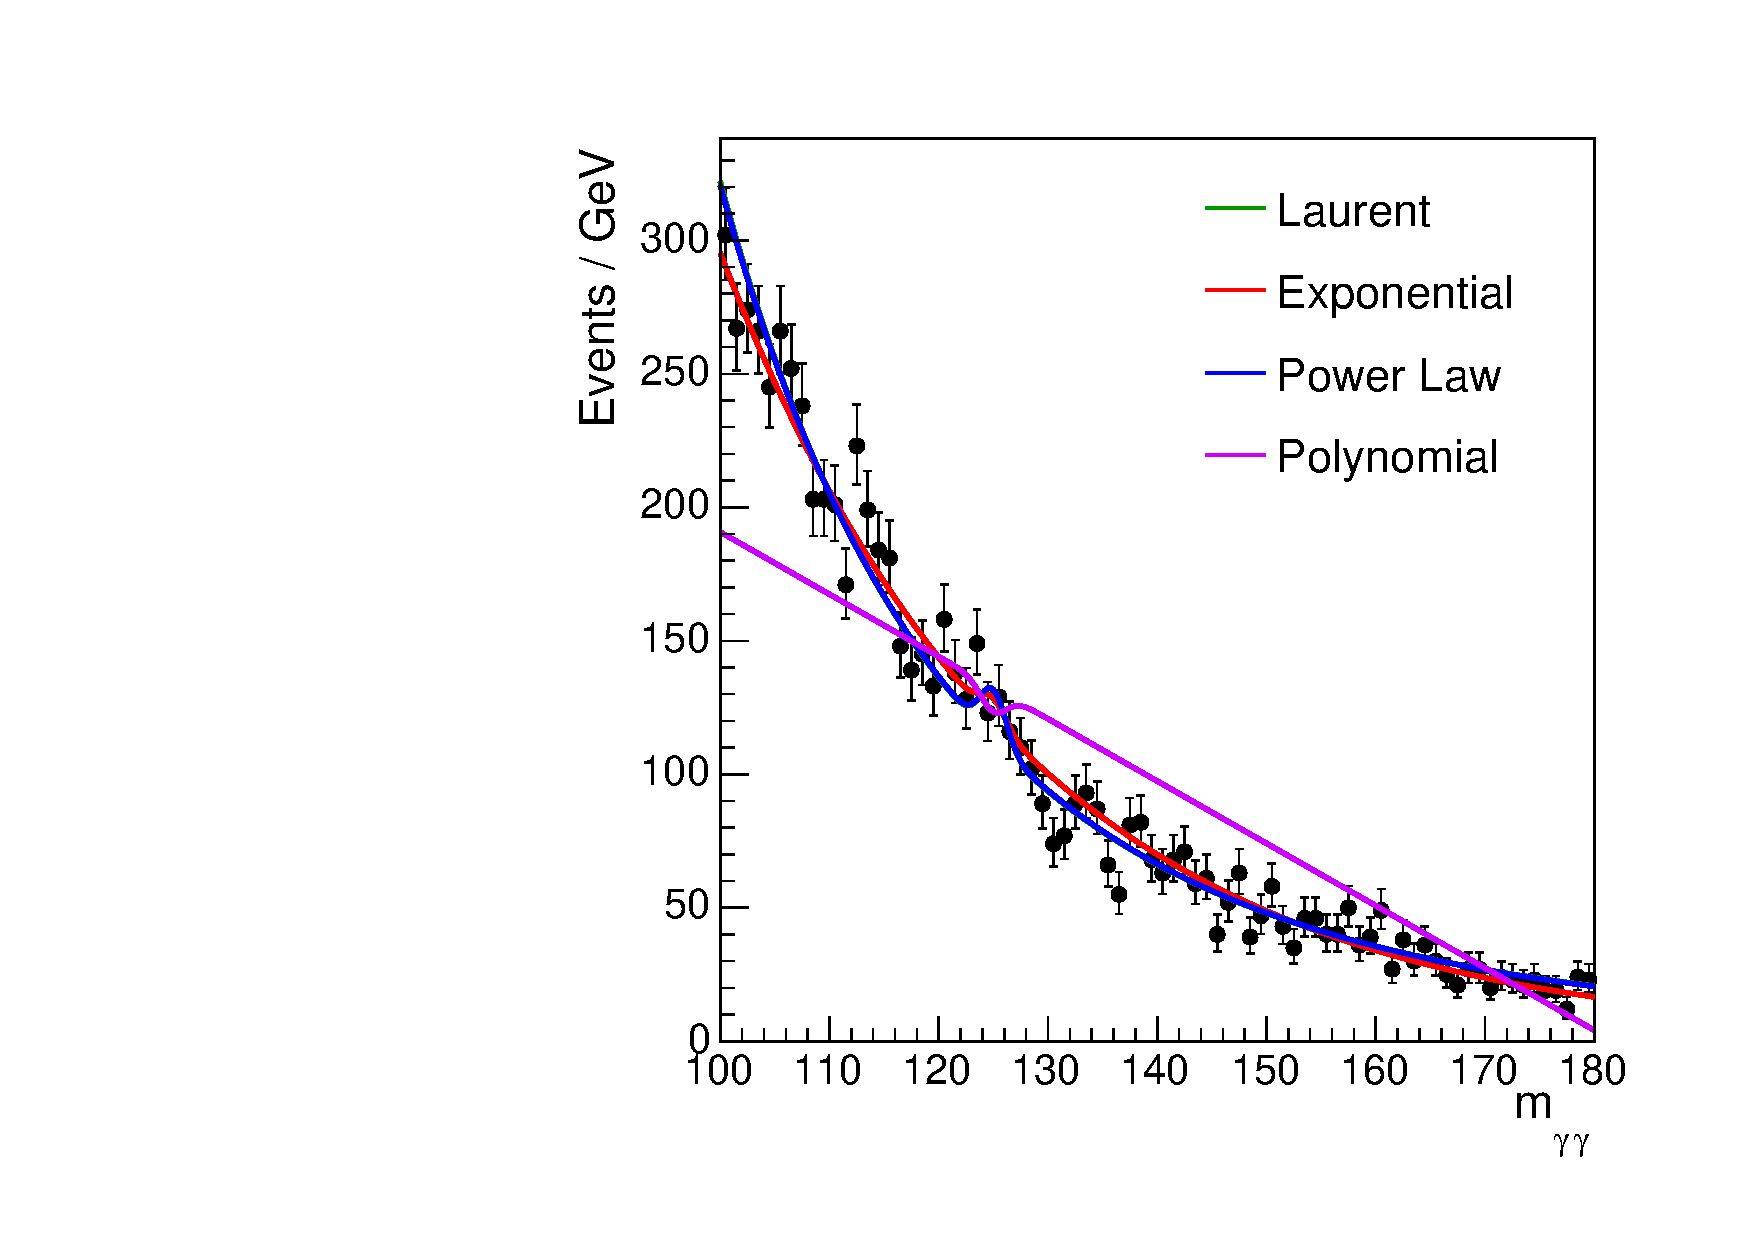
\includegraphics[width=0.45\textwidth]{functions/BestFits.pdf}
\caption{Best fits of the four two-parameter functions (described in the
text). The dashed lines indicate the background component of the fit while the solid lines include  
the signal component. The Laurent function is effectively identical to the power law function
and so is hidden below the power law line. Note, for clarity in this plot, the
data have been rebinned into 40 bins, although the fits were done with the
fine 160 binning.}
\label{fig:functions:bestfits}
\end{figure}

The profile scan as a function of the relative signal strength $\mu$
between $-1.0$ and 2.5
for the four functions is shown in
figure~\ref{fig:functions:profiles}.
The absolute minimum occurs for the power law function at a relative signal 
strength of $\mu = 0.93$. If just considering this function,
then one would set a 68.3\% confidence interval on $\mu$ of  
$0.43 < \mu < 1.40 $, determined as the interval for which $\Delta({\rm \nll}) < 1$. 
The measurement would therefore be reported with its standard error as $\mu=0.93^{+0.47}_{-0.50}$. The Laurent function gives an almost identical result.
When fitting the exponential function a very similar \nll value is obtained
at its best fit, but gives a best relative signal strength of $\mu = 0.72$
and a 68.3\% confidence interval of
$0.27 < \mu < 1.24 $, which would be quoted as $\mu = 0.72^{+0.52}_{-0.45}$.
Fitting with the straight line yields a very different result of 
$\mu = 0.01^{+0.51}_{-0.47}$ 
although its clear that this function does not describe the data well.
The fact that the different functions can give different best fit values
is a direct example of the systematic error associated
with the choice of function.
%
\begin{figure}[tbp]
\centering
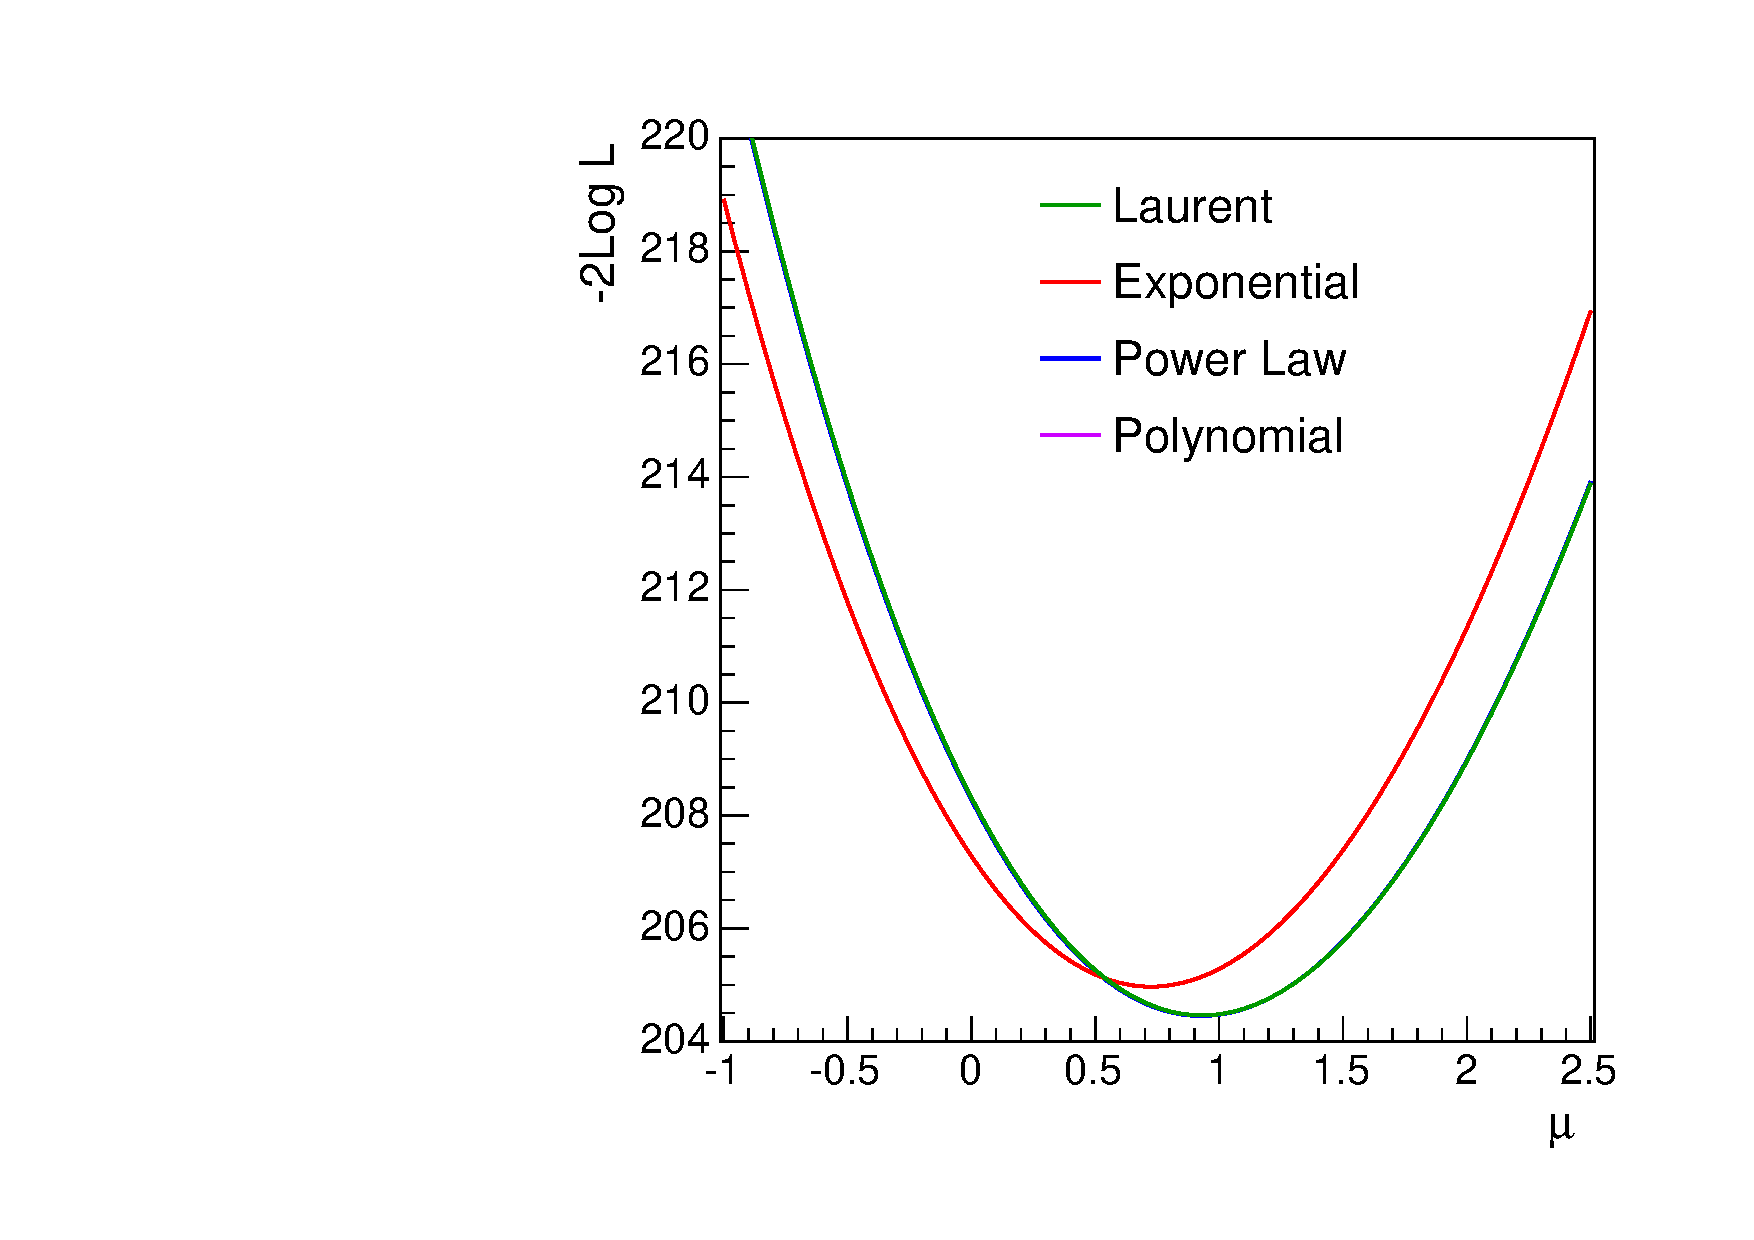
\includegraphics[width=0.45\textwidth]{functions/Profiles.pdf}
\caption{Profile \nll scans for the four functions discussed in the text.
The polynominal function is always above the top of the \nll scale shown in this
figure. }
\label{fig:functions:profiles}
\end{figure}

The envelope around these functions is shown in
figure~\ref{fig:functions:envelope}.
As it has to be, the best fit is still $\mu=0.93$ from the power law
but now the standard error is enlarged by the exponential function
contribution to the
envelope on the lower side of the scan. Hence, taking all four functions into
account, the 68.3\% confidence interval on $\mu$ is
$0.27 < \mu < 1.40 $, i.e. the lower limit from the exponential fit and the
upper limit from the power law fit,
and the measured value of $\mu$ which would now be quoted is 
$\mu = 0.93_{-0.56}^{+0.47}$.
The enlarged uncertainty is a direct reflection of the
systematic error arising from the function uncertainty.
As also shown in figure~\ref{fig:functions:envelope}, the 95.4\% confidence 
interval is $-0.18 < \mu < 1.92$.
Note, it is clear that the poor fit of the polynomial
means it plays no role in the envelope and so this function is 
``automatically'' ignored by the method,
without requiring any arbitrary criterion for
including it or not.
%
\begin{figure}[tbp]
\centering
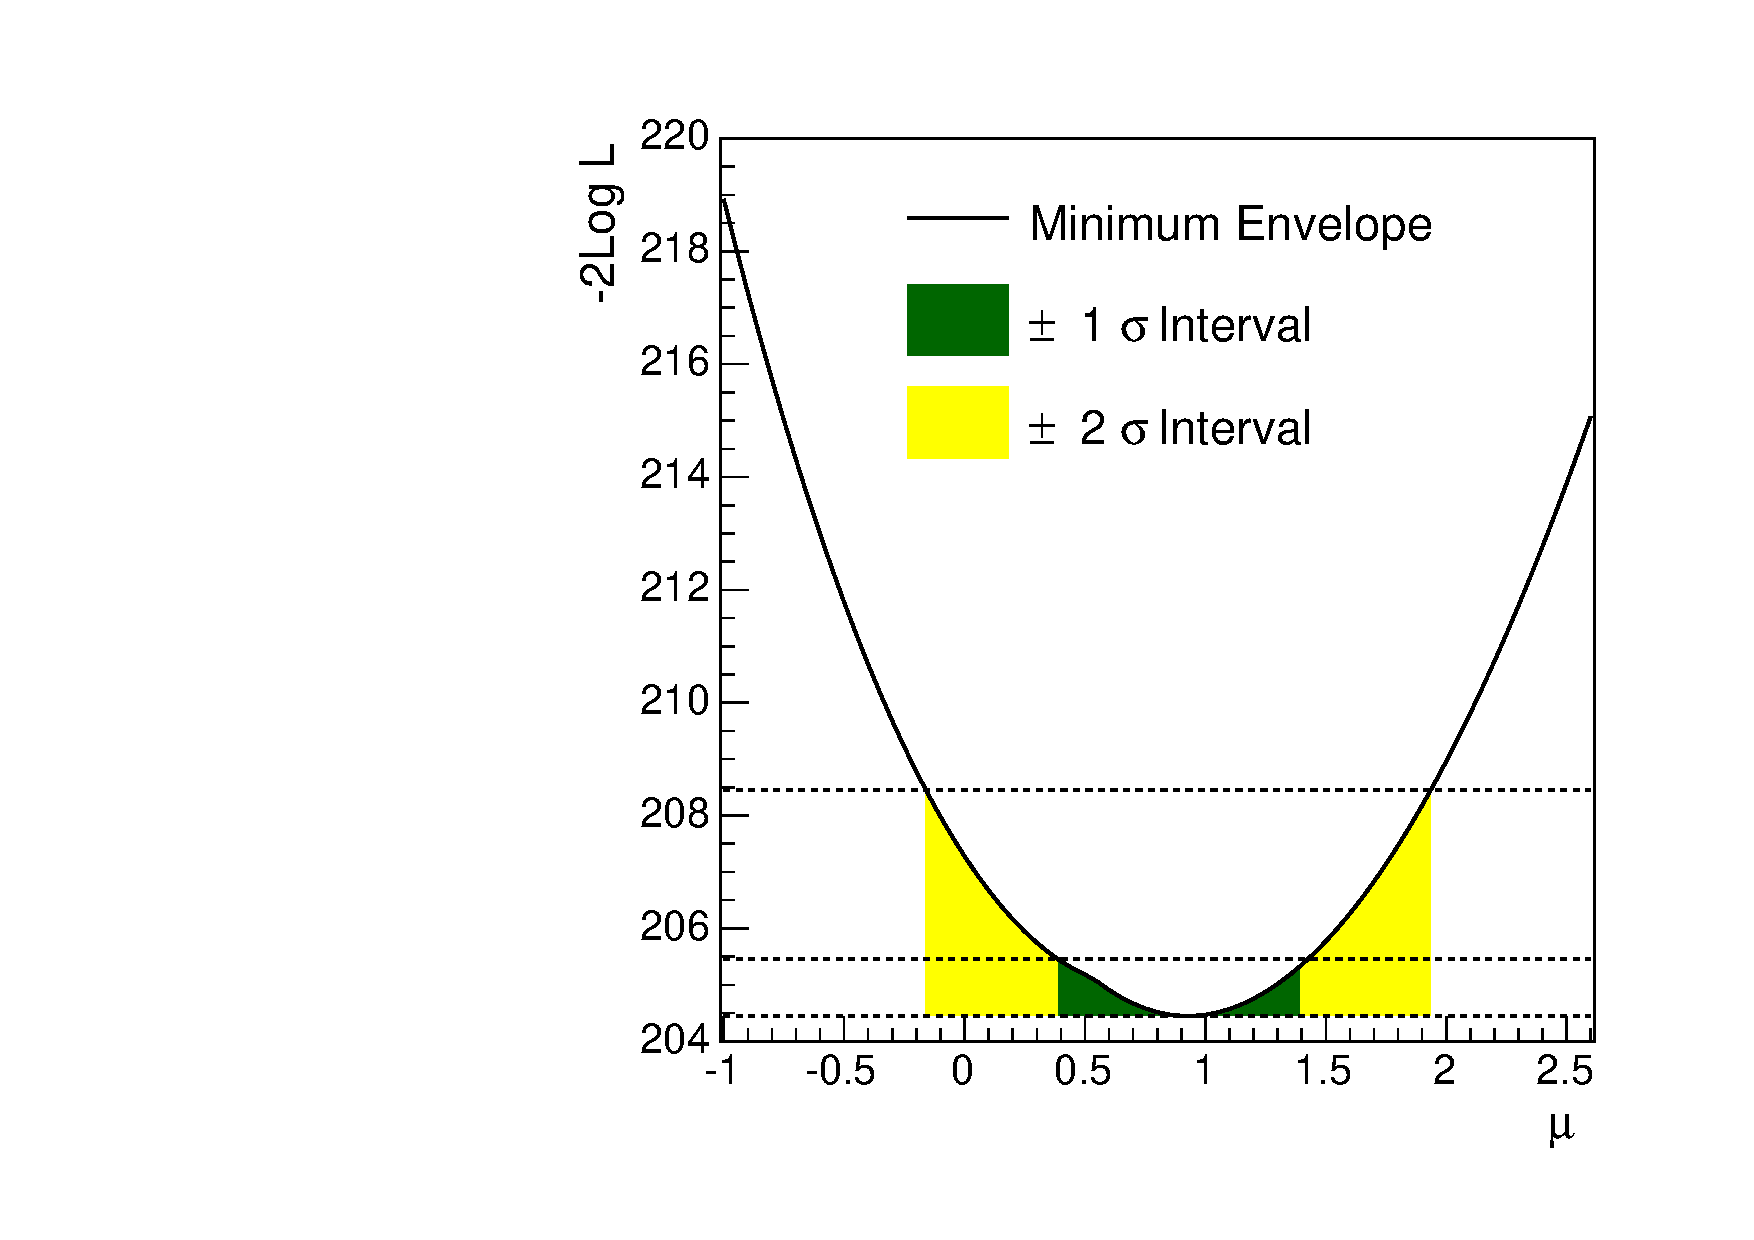
\includegraphics[width=0.45\textwidth]{functions/Envelope.pdf}
\caption{Profile \nll envelope for the four two-parameter function fits.
The coloured bands indicate the $1\sigma$ and $2\sigma$ intervals determined from the regions 
for which the value of \nll increases by 1 and 4 units from the minimum value as indicated by the horizontal lines.}
\label{fig:functions:envelope}
\end{figure}


\subsection{Bias and coverage}
\label{sec:functions:coverage}

The discrete profile method was tested for bias and coverage 
using a large ensemble of
pseudo-experiments (``toys''). For each of these, a toy
dataset including signal and background events generated using a Monte Carlo technique. 
The background function was chosen to be one of the four two-parameter functions discussed above, with
the parameters set to their best fit values for each value of $\mu$.
Several ensembles of toy pseudo-experiments were 
generated varying the normalization of the signal function in order to test the properties 
of the method as a function of the parameter $\mu$.  

In addition, a further ensemble of toy datasets was generated, for which the
background function itself, as well as its parameters, was chosen according to
the best fit for each value of $\mu$. From figure~\ref{fig:functions:profiles},
it can be seen that this means the exponential function is used for $\mu<0.55$
and the power law function is used otherwise. Conceptually, this method again
treats the function choice as a discrete nuisance parameter and so picks the
best fit values of all parameters for each $\mu$ value.

In all cases, the resulting toy datasets were then treated identically to the
original dataset, with a fit for the relative signal strength using
each of the four functions as background, and then forming the envelope.
For each ensemble of datasets, the mean pull of the relative
signal strength was determined. Figure~\ref{fig:functions:firstorderbias}
shows the result of these fits. It is seen that the envelope gives a
relatively small
bias ($\sim 0.1\sigma$) for all cases, 
which is not the case when choosing to use
any one specific function.
%
\begin{figure}[tbp]
\centering
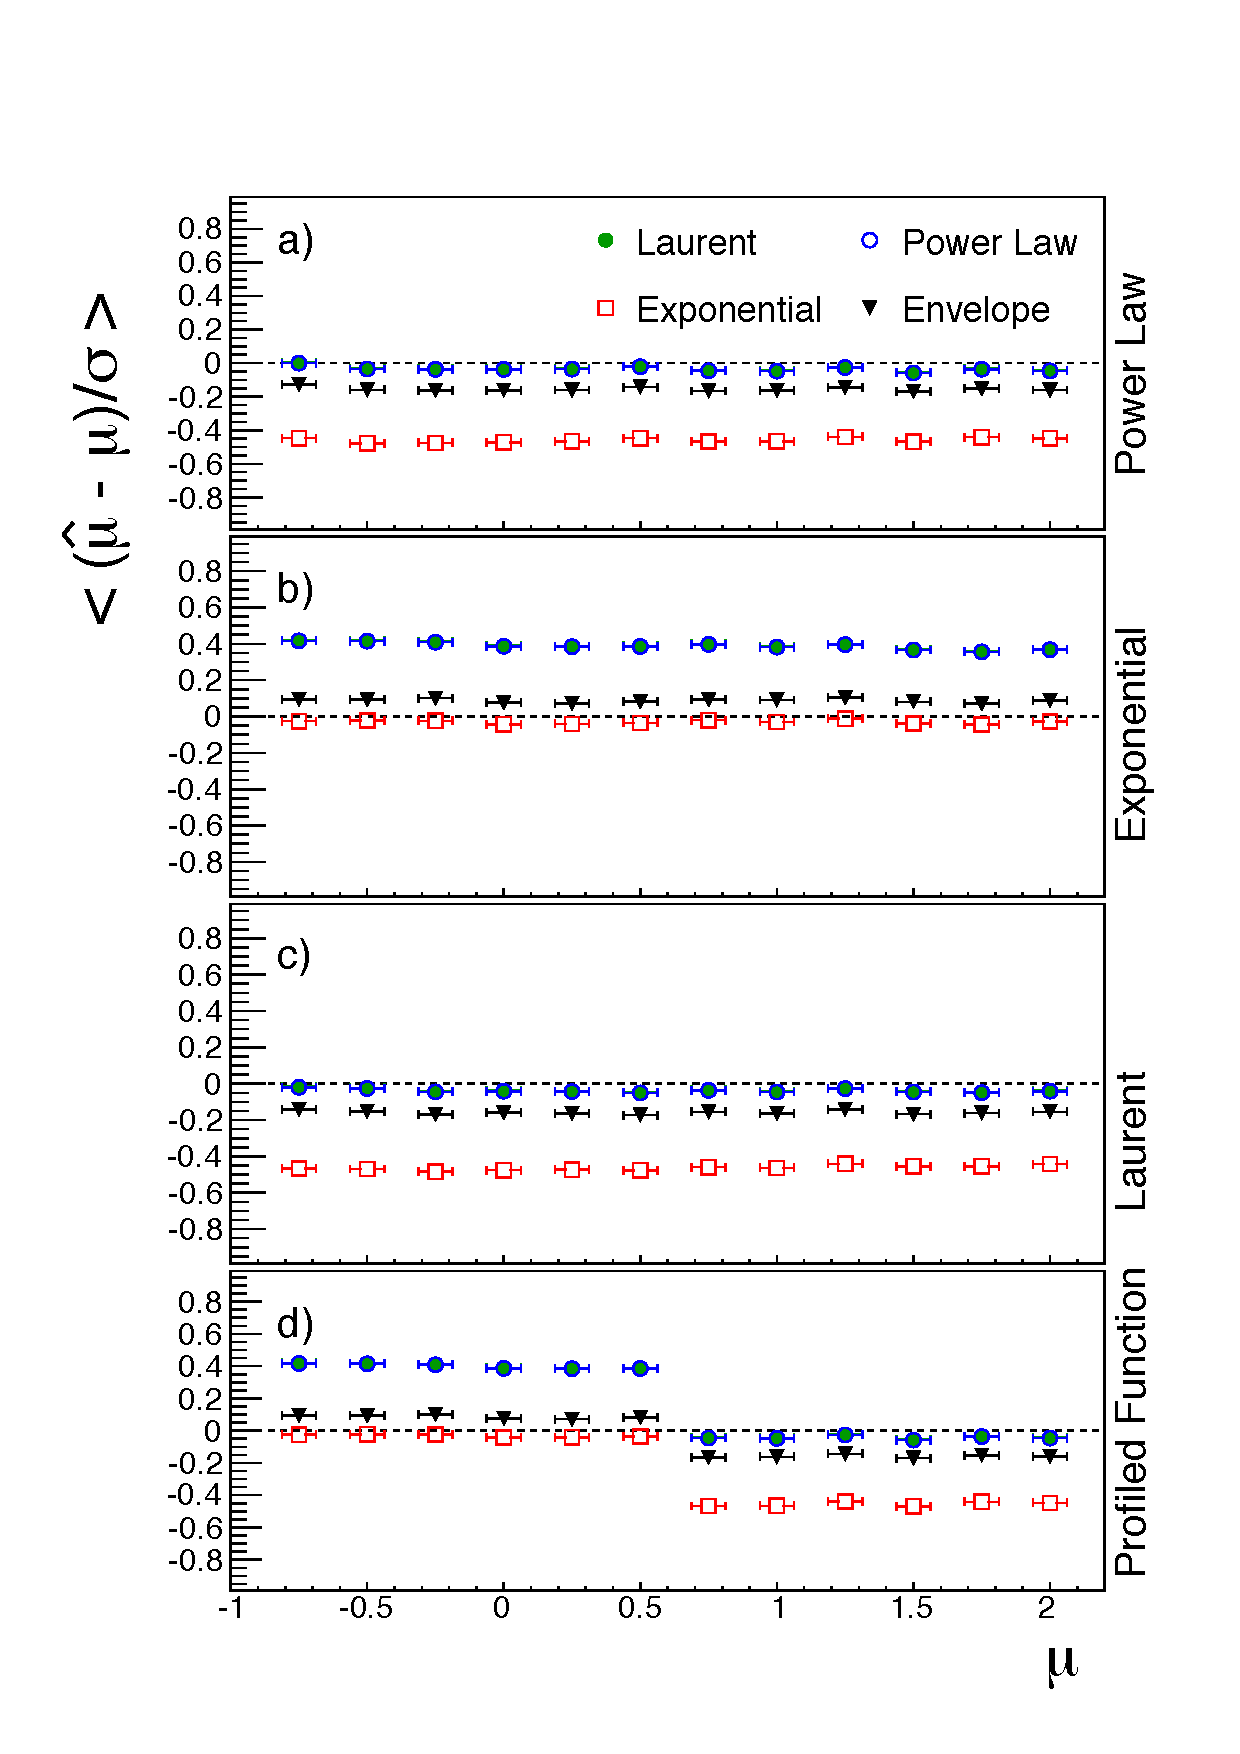
\includegraphics[width=0.45\textwidth]{functions/FirstOrderFunctions.pdf}
\caption{Average pull when fitting with each function as background and when
using the envelope. The first, second and third plots shows the results
when the generating background function is power law, exponential and Laurent,
respectively. The lowest plot show the result when the best-fit function at each
value of $\mu$ is used to generate toys; this means the exponential function
below $\mu = 0.55$ and the power law function above this value. In all cases,
the polynomial gives values outside the range of these plots.}
\label{fig:functions:firstorderbias}
\end{figure}

% COMMENT ON BIAS FROM DISCRETE PARAMETER SPACE!

The coverage was also determined from the same fits. The difference of the
\nll between the best fit value and the true value of the relative signal 
strength was found and the fraction of times this was less than 0.25, 1, 4 and 9, was
determined. Figure~\ref{fig:functions:firstordercoverage}
shows the result of these studies. It is seen that the envelope gives good
coverage for all cases, which is again not the case for any of the specific 
functions.
%
\begin{figure}[tbp]
\centering
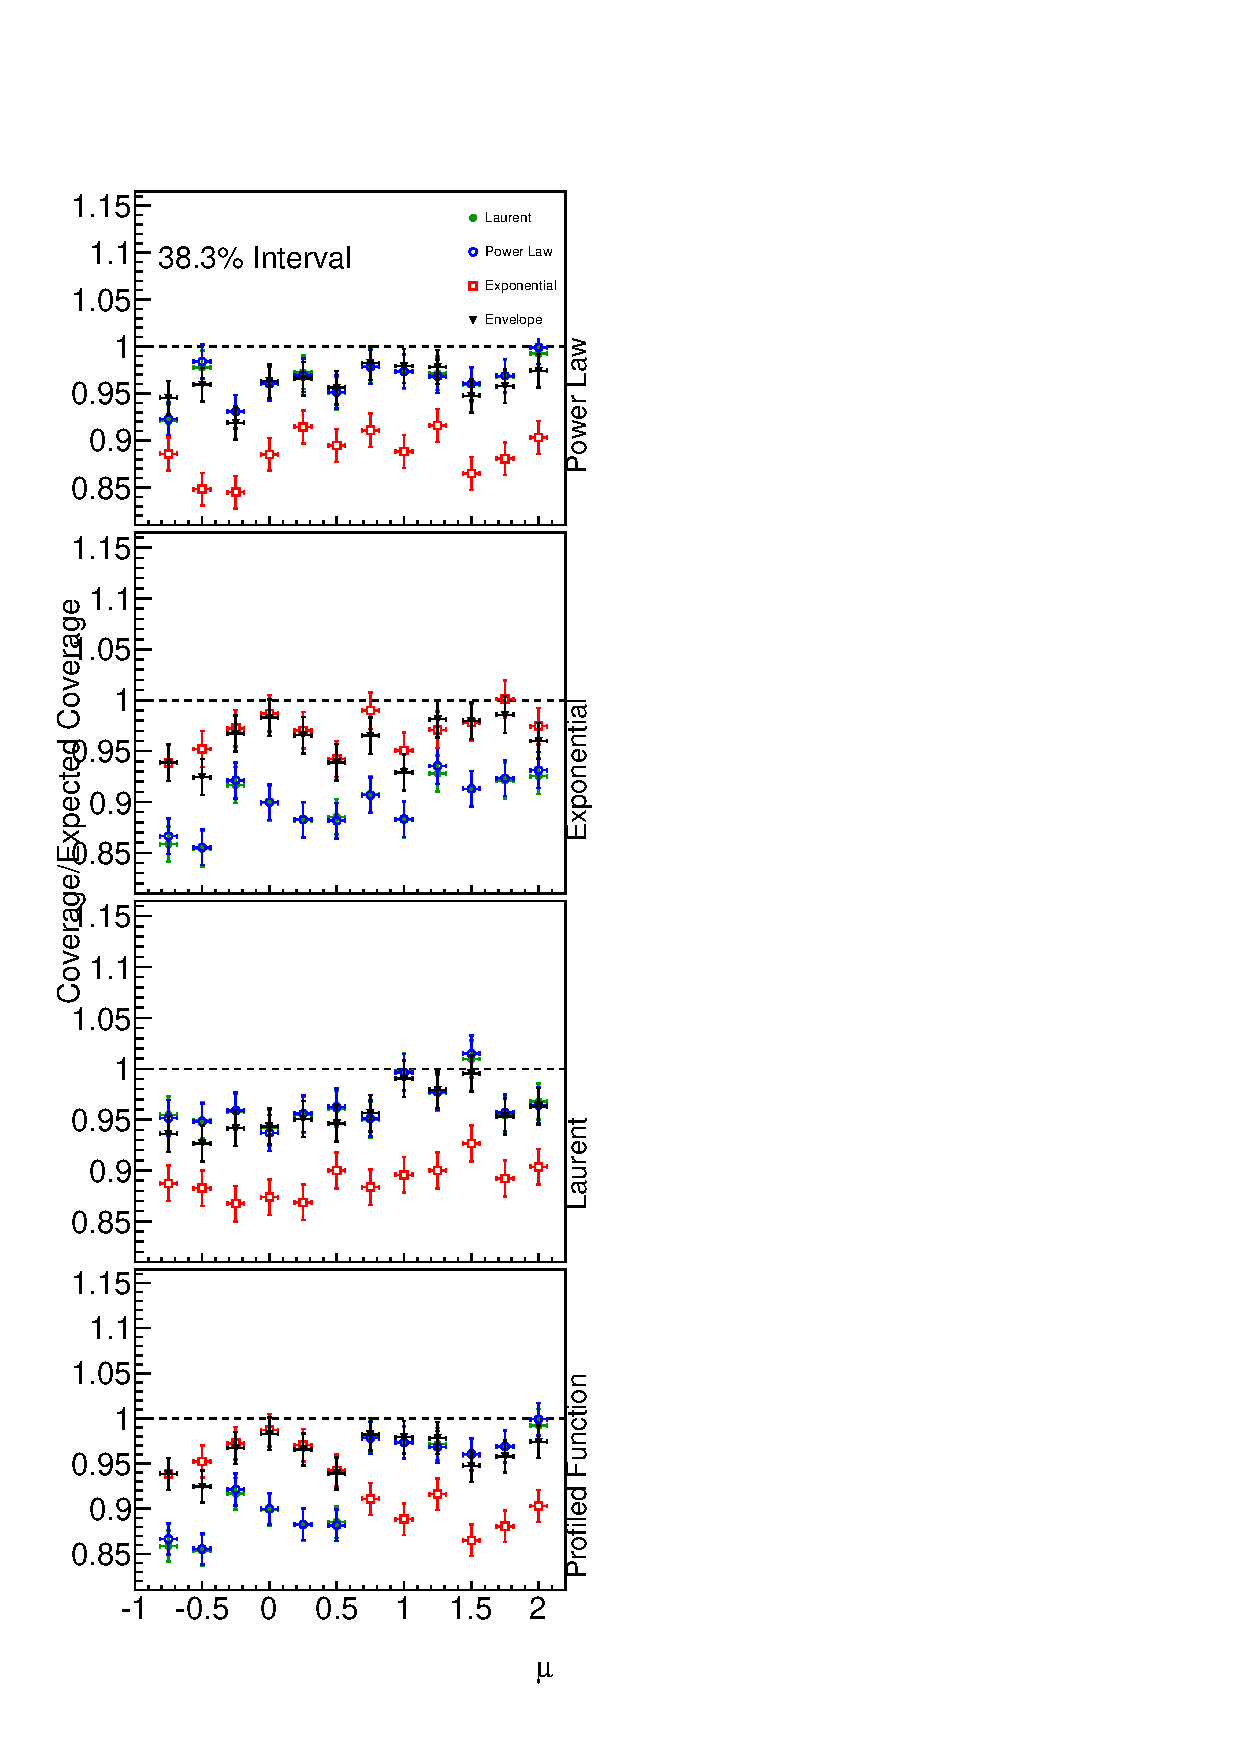
\includegraphics[width=0.45\textwidth]{{functions/FirstOrderFunctions_Coverage_0.5}.pdf}
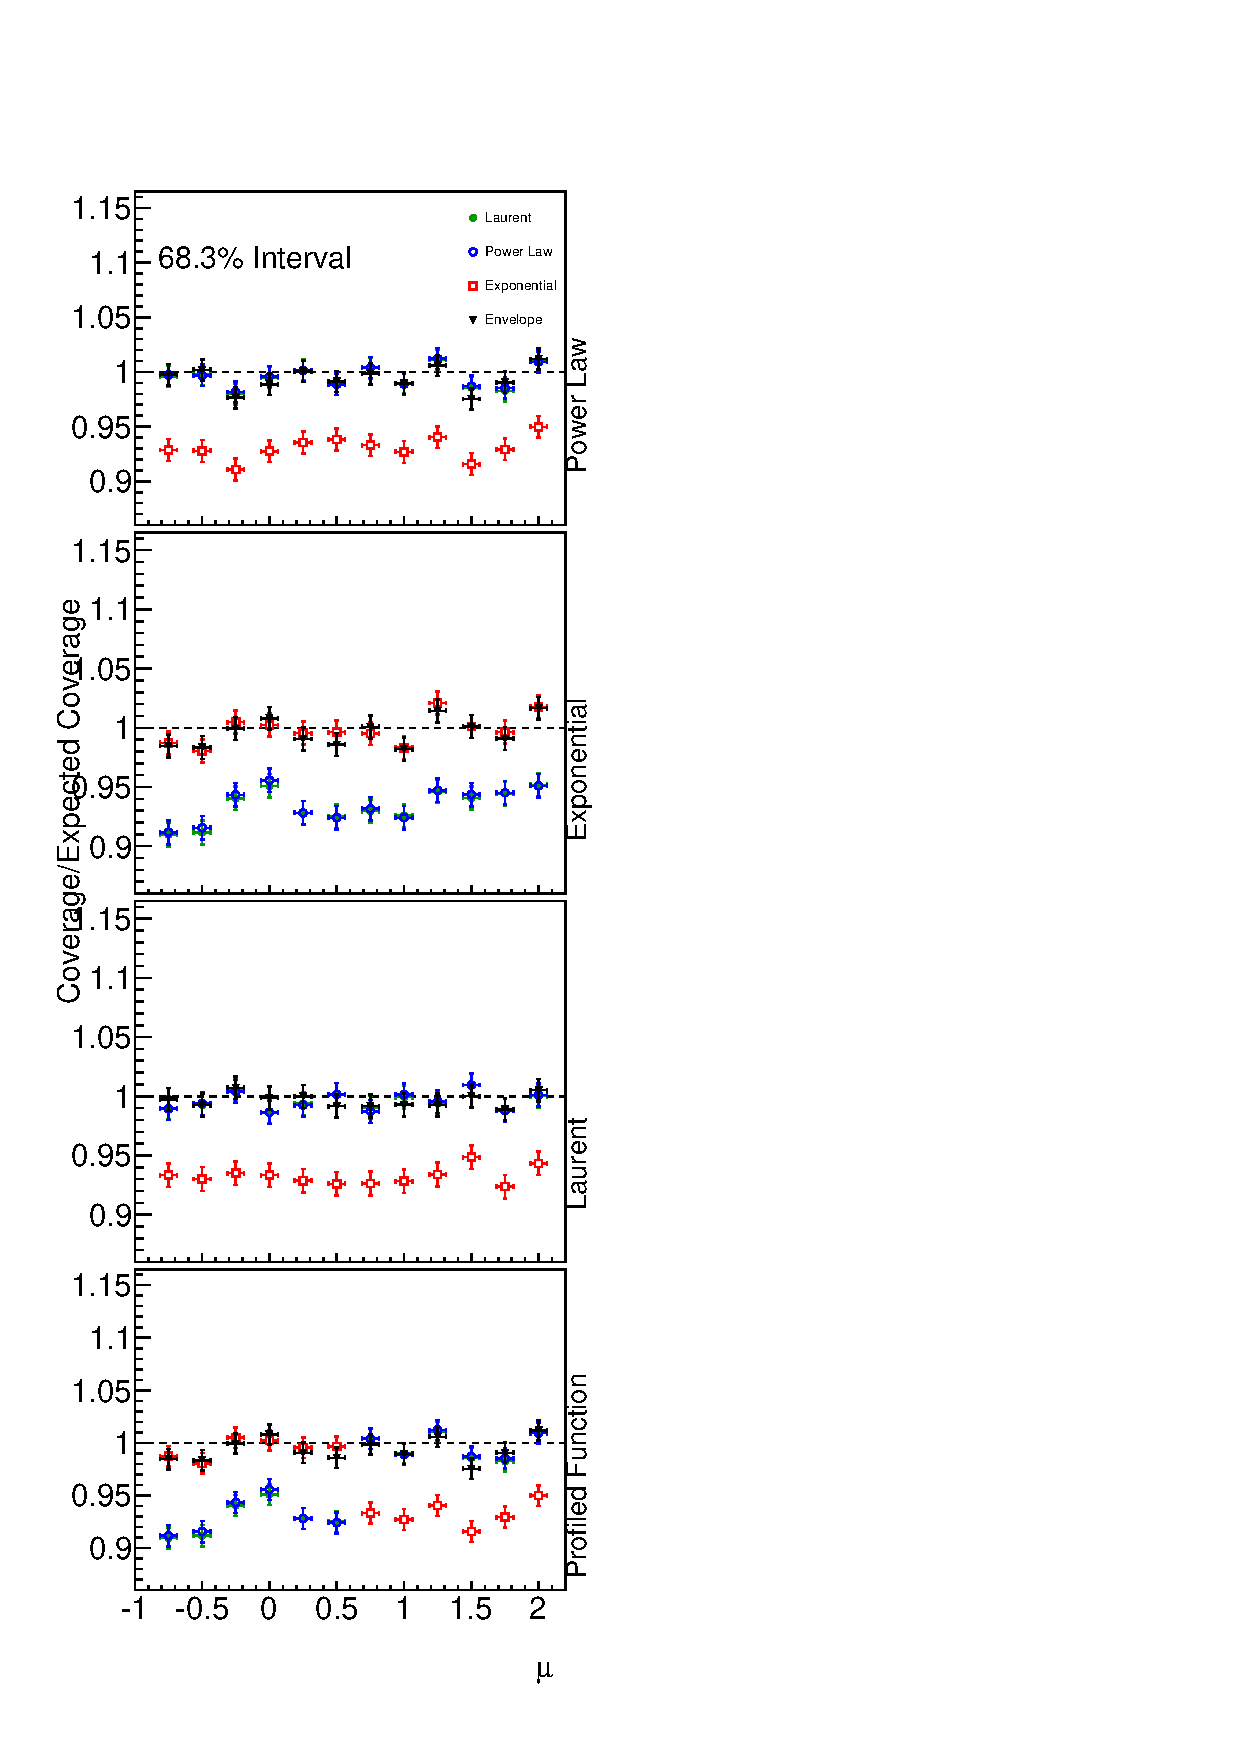
\includegraphics[width=0.45\textwidth]{{functions/FirstOrderFunctions_Coverage_1.}.pdf}\\
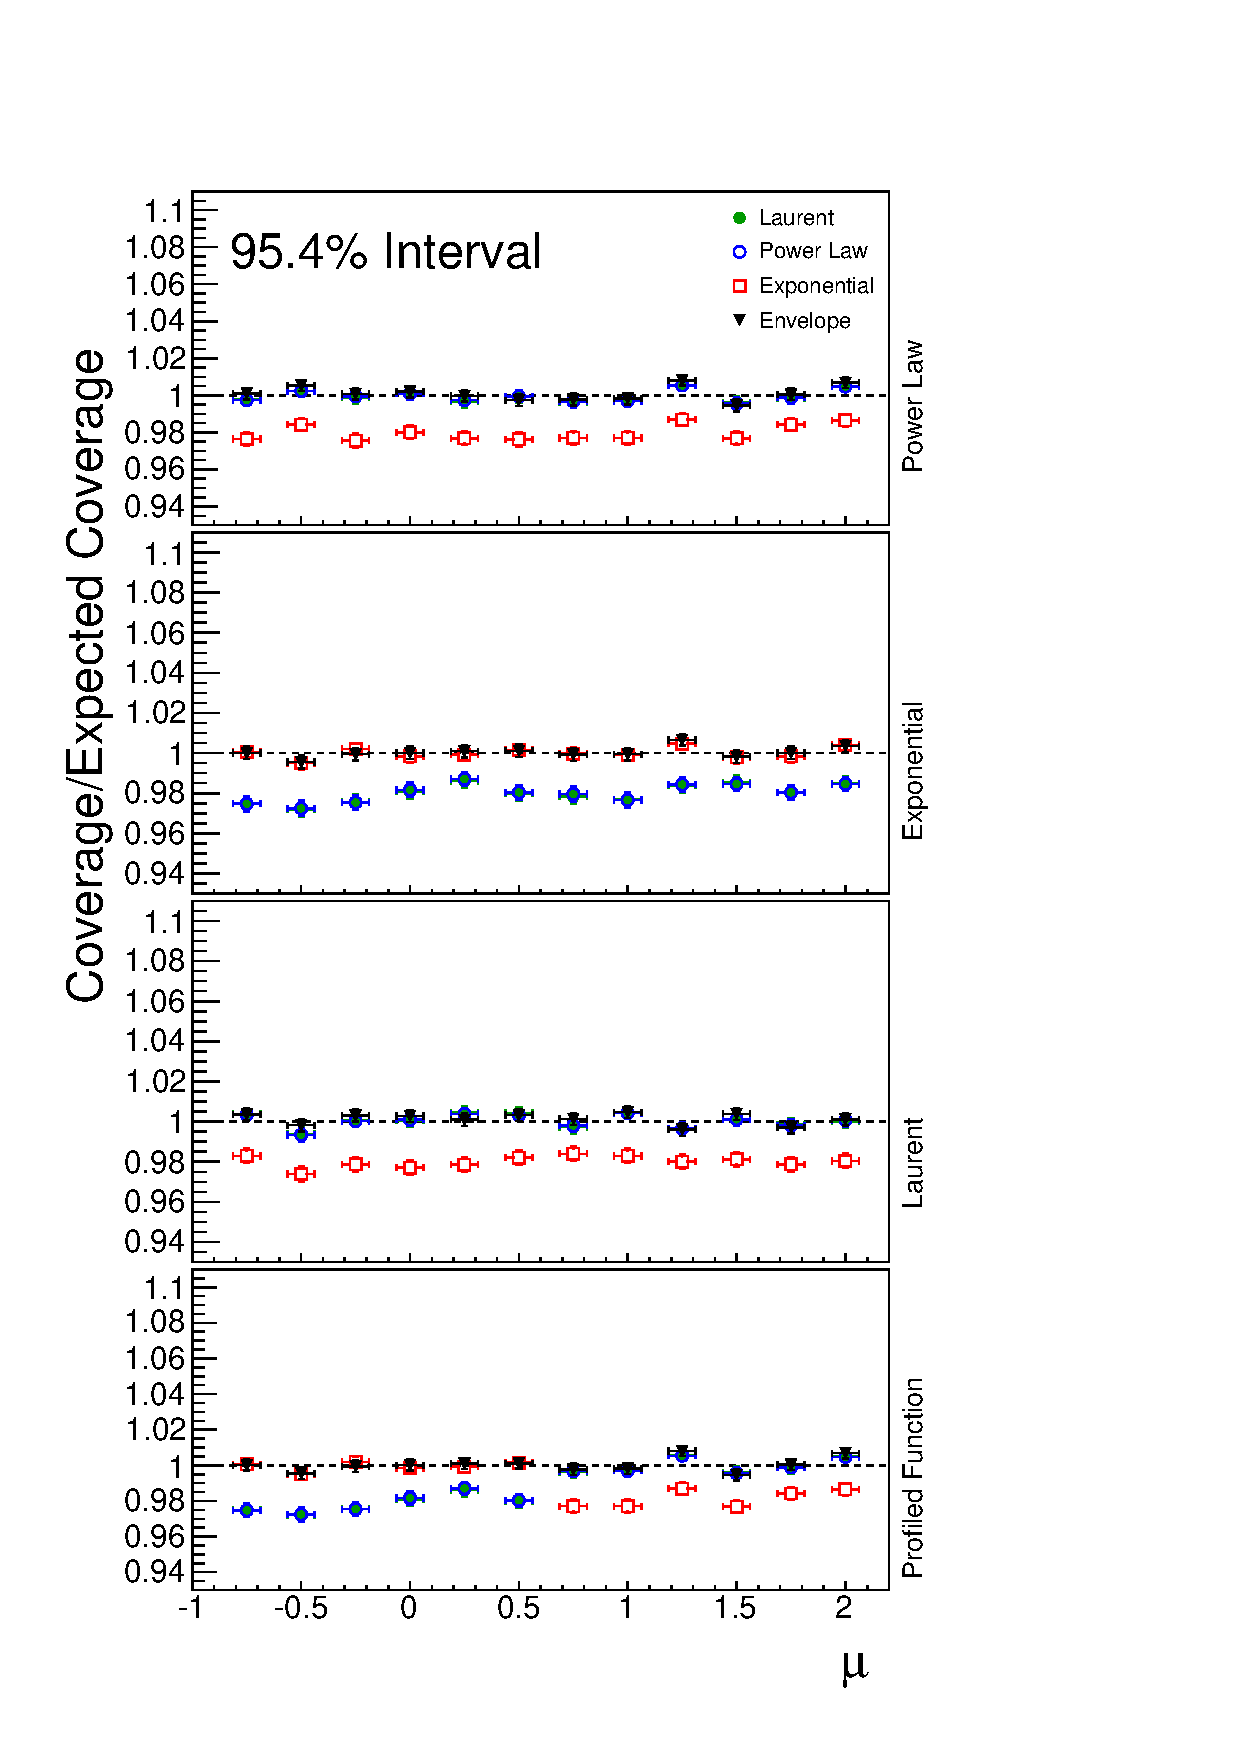
\includegraphics[width=0.45\textwidth]{{functions/FirstOrderFunctions_Coverage_2.}.pdf}
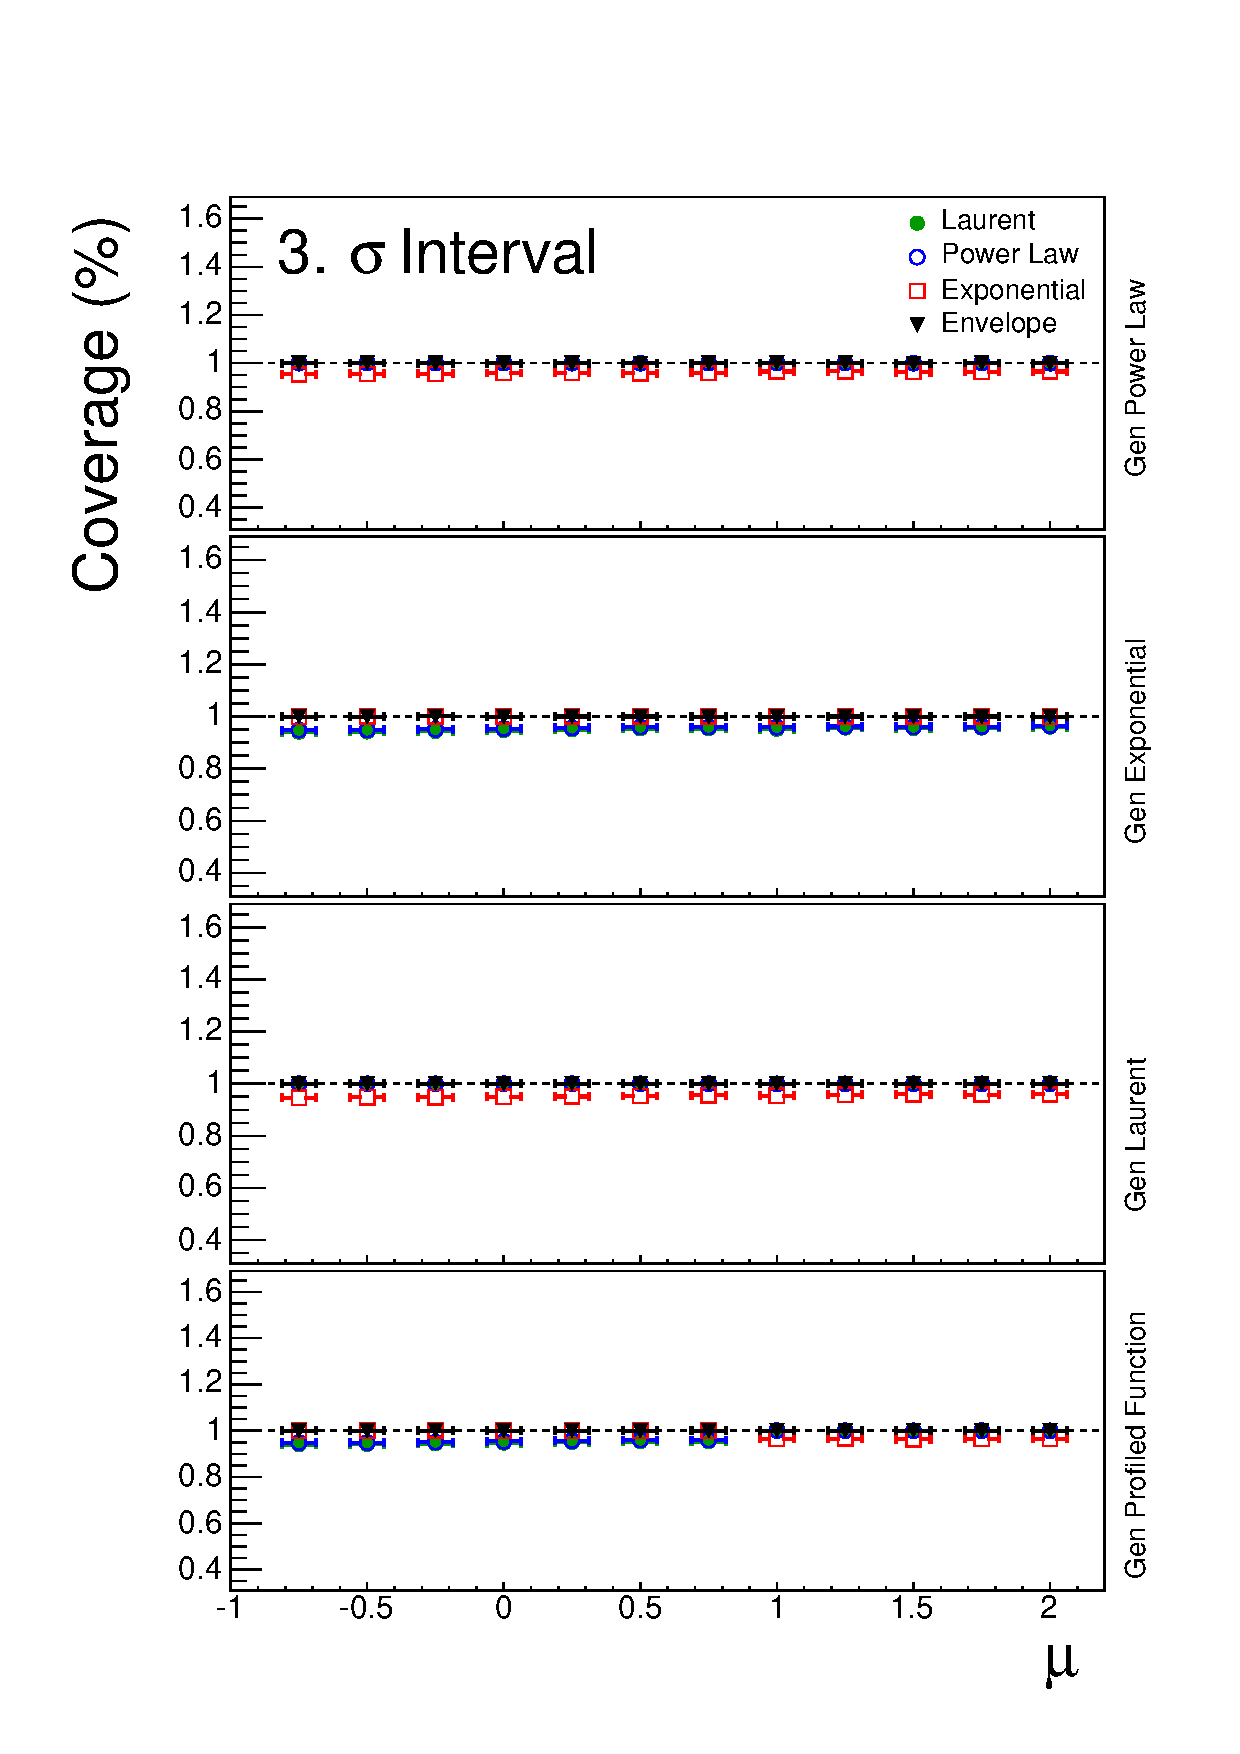
\includegraphics[width=0.45\textwidth]{{functions/FirstOrderFunctions_Coverage_3.}.pdf}
\caption{Fraction of toys in which the fitted value of $\mu$ is within the 0.5, 1, 2 and 
$3\sigma$ intervals relative to the expected fraction for that interval using a single 
function and using the envelope.
Within each subfigure,
the first, second and third plots shows the results
when the generating background function is power law, exponential and Laurent,
respectively. The lowest plot in each subfigure
show the result when the best-fit function at each
value of $\mu$ is used to generate toys.}
\label{fig:functions:firstordercoverage}
\end{figure}


%ASIMOV RESULTS AS PART OF DISCUSSION ON BIAS?

%UNBINNED MENTIONED ONLY IN PASSING


%\subsection{Toy generation}
%\label{sec:functions:toys}

%WHAT IS A BETTER TERM THAN ``TOYS''?

%1. USING SINGLE FUNCTION (GIVING BIAS)

%2. USING BAYESIAN PROBABILITY MIX OF FUNCTIONS (NO BIAS)

%3. USING FREQUENTIST FRACTIONAL CONTRIBUTIONS OF FUNCTIONS (BIAS???)
